\chapter{Disseny del sistema}

\section{M�duls}
Hem organitzat el codi del sistema en els seg�ents m�duls:
\begin{itemize}
\item{\textit{Raw Content Extraction} (rce):}
Agrupa totes les classes encarregades d'extreure el contingut dels documents PDF.

\item{\textit{Information Retrieval} (ir):}
Encarregat de comunicar-se amb els diferents cercadors disponibles a Internet per obtenir p�gines que contenen informaci� de la refer�ncia que volem extreure.

\item{\textit{Information Extraction} (ie):}
Cont� tot el codi que permet obtenir la refer�ncia a partir d'una p�gina HTML. A m�s, tamb� �s l'encarregat de generar nous \textit{wrappers}.

\item{\textit{References}:}
Per una banda fa un an�lisis sint�ctic de les refer�ncies extretes per poder-les validar. Per l'altra, transforma a \BibTeX les refer�ncies extretes.

\item{Base de dades (db):}
Tal i com indica el seu nom, duu a terme els accessos la base de dades.

\item{\textit{Main}: }
Enlla�a tots els m�duls anteriors i proporciona punts d'entrada a la interf�cie d'usuari. Fa de fa�ana del sistema.

\item{\textit{Graphical User Interface} (gui):}
Interf�cie d'usuari m�s o menys amigable.
\end{itemize}

La figura \ref{fig:module_diagram} mostra com interaccionen entre ells.

\begin{figure}[h!]
\begin{center}
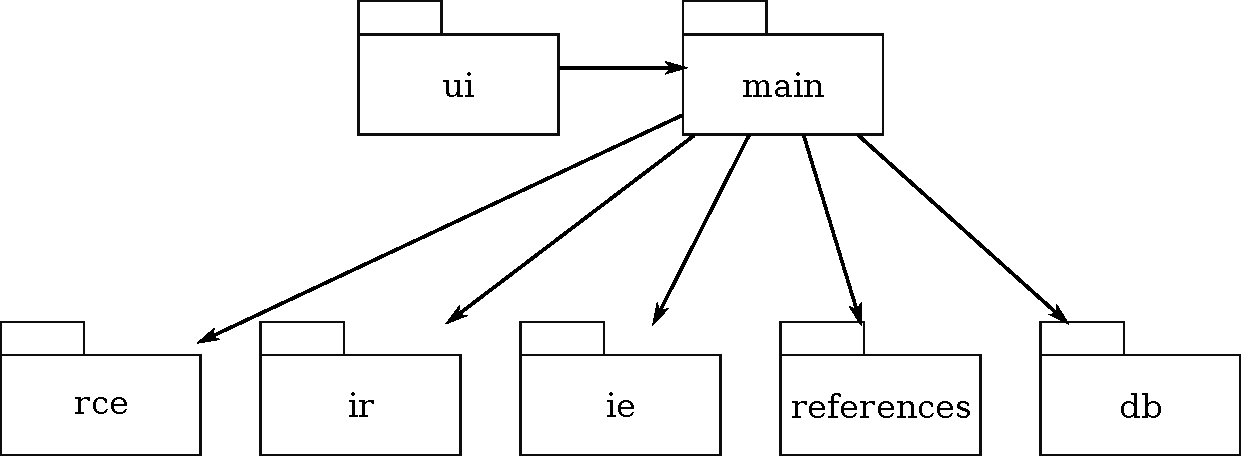
\includegraphics[width=0.6\textwidth]{figures/module_diagram.pdf}
\caption{M�duls del sistema}
\label{fig:module_diagram}
\end{center}
\end{figure}
